\documentclass{article}
\usepackage{cmap}
\usepackage[utf8]{inputenc}
\usepackage[english,ukrainian]{babel}
\usepackage{graphicx}
\usepackage{geometry}
\usepackage{listings}
\usepackage{float}
\usepackage{amsmath}
\geometry{
	a4paper,
	left=20mm,
	right=20mm,
	top=15mm,
	bottom=15mm,
}
\lstset{
	language=c,
	tabsize=4,
	keepspaces,
	showstringspaces=false,
}
\graphicspath{ {./pictures} }
\setlength{\parindent}{4em}

\newcommand\subject{Програмування в Інтернет}
\newcommand\lecturer{асистент кафедри ПЗ \\ Степанов Д.С.}
\newcommand\teacher{доцент кафедри ПЗ \\ Грицай О.Д.}
\newcommand\mygroup{ПЗ-22}
\newcommand\lab{4}
\newcommand\theme{Основні типи та функції доступу до БД MySQL}
\newcommand\purpose{Засвоїти елементи створення, модифікації, читання та занесення даних з таблиць БД засобами РНР}

\begin{document}
\begin{normalsize}
\begin{titlepage}
	\thispagestyle{empty}
	\begin{center}
		\textbf{МІНІСТЕРСТВО ОСВІТИ І НАУКИ УКРАЇНИ\\
			НАЦІОНАЛЬНИЙ УНІВЕРСИТЕТ "ЛЬВІВСЬКА ПОЛІТЕХНІКА"}
	\end{center}
	\begin{flushright}
		\textbf{ІКНІ}\\
		Кафедра \textbf{ПЗ}
	\end{flushright}
	\vspace{200pt}
	\begin{center}
		\textbf{ЗВІТ}\\
		\vspace{10pt}
		до лабораторної роботи № \lab\\
		\textbf{на тему}: “\textit{\theme}”\\
		\textbf{з дисципліни}: “\subject”
	\end{center}
	\vspace{112pt}
	\begin{flushright}
		
		\textbf{Лектор}:\\
		\lecturer\\
		\vspace{28pt}
		\textbf{Виконав}:\\
		
		студент групи \mygroup\\
		Коваленко Д.М.\\
		\vspace{28pt}
		\textbf{Прийняв}:\\
		
		\teacher\\
		
		\vspace{28pt}
		«\rule{1cm}{0.15mm}» \rule{1.5cm}{0.15mm} 2023 р.\\
		$\sum$ = \rule{1cm}{0.15mm}……………\\
		
	\end{flushright}
	\vspace{\fill}
	\begin{center}
		\textbf{Львів — 2023}
	\end{center}
\end{titlepage}
	
\begin{description}
	\item[Тема.] \theme.
	\item[Мета.] \purpose.
\end{description}

\section*{Індивідуальне завдання}
Розробити web-сторінку згідно макета (wireframe)
https://cacoo.com/diagrams/ZvVhYS3UpG5PdbBy/EDE3A
Обираємо для розробки шаблон Students Add/Edit
Використовуємо Gitlab (https://gitlab.com)
Сторінка має містити:\\
- Сайт з формою, що надсилає на сервер дані студента\\
- Серверна частина перевіряє чи наявні та коректні всі поля і повертає інформацію у json форматі\\
- айт реагує на відповіді. Якщо прийшла помилка відображає, якщо немає помилки додає у
таблицю студента\\

\section*{Теоретичні відомості}
Одним з інструментів підтримки динамічних сценаріїв при перегляді Web-сторінок у
межах комп’ютера користувача є мова програмування JavaScript – спрощений
варіант мови програмування Java. Нею запезпечується рух об’єктів на сторінці,
введення та виведення параметрів, зміна зображень вікон тощо. Програми модифікації,
створення гіпертекстових сторінок традиційно називають скриптами (scripts), які
інтерпретуються програмою перегляду. Спосіб базується на ідеології об’єктно-
орієнтованого програмування. Зупинимось на скриптах, написаних мовою JavaScript.

Усі операції в програмі на JavaScript описують дії над об’єктами – елементами
робочої області броузера та контейнерами мови HTML. Об’єкти мають властивості та
методи. Існують також інші функції, які дають змогу працювати зі стандартними
математичними функціями та керувати процесом виконання програми. JavaScript має
механізм опрацювання подій перегляду динамічних об’єктів та управління
багатовіконним інтерфейсом. Об’єкти JavaScript беруть свій початок від класу
Window.

Bootstrap – це фреймворк для розробки клієнтських застосувань (front end). Bootstrap
містить шаблони на базі HTML та CSS з текстом, формами, кнопками, таблицями,
навігацією, модулями, каруселями зображень та багато інших сучасних елементів веб
сторінок, а також вбудовані засоби JavaScript (плагіни). Bootstrap дозволяє створювати
адаптивні сторінки у телефонах, планшетах та ноутбуках.. Bootstrap 3 підтримує
реалізацію для мобільних телефонів. Bootstrap підтримується у сучасних браузерах
(Chrome, Firefox, Internet Explorer, Safari, Opera). Версія 4.0 містить препроцесор CSS
(SASS ) та підтримку flex-box.

\section*{Хід виконання}
\begin{lstlisting}
<?php
if ($_SERVER['REQUEST_METHOD'] === 'POST') {
	$json = file_get_contents('php://input');
	$student = json_decode($json);
	
	$id = trim($student->id);
	$group = trim($student->group);
	$name = trim($student->name);
	$gender = trim($student->gender);
	$birthday = trim($student->birthday);
	$status = trim($student->status);
	
	$errors = [];
	
	if (empty($id)) {
		$errors[] = 'ID is required.';
	}
	
	if (empty($group)) {
		$errors[] = 'Group is required.';
	}
	
	if (empty($name) || strlen($name) < 5) {
		$errors[] = 'Name is required and should be at least 5 characters in length.';
	}
	
	if (empty($gender) || !in_array($gender, ['Male', 'Female', 'Other'])) {
		$errors[] = 'Gender is required and must be "male", "female", or "other".';
	}
	
	if (empty($birthday)) {
		$errors[] = 'Birthday is required.';
	} elseif (!preg_match('/^\d{4}-\d{2}-\d{2}$/', $birthday)) {
		$errors[] = 'Birthday must be in the format "YYYY-MM-DD".';
	}
	
	if (empty($status) || !in_array($status, ['0', '1'])) {
		$errors[] = 'Status is required and must be "0" or "1".';
	}
	
	if (!empty($errors)) {
		http_response_code(400);
		echo json_encode(['errors' => $errors]);
		exit;
	} else {
		http_response_code(200);
		exit;
	}
}
?>

\end{lstlisting}

\section*{Результати}
\begin{figure}[H]
	\centering
	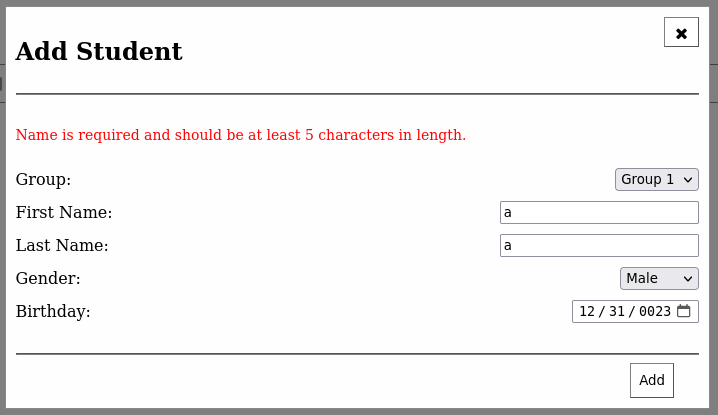
\includegraphics[scale=0.35]{23}
	\caption{Валідація даних серверною частиною.}
\end{figure}

\begin{figure}[H]
	\centering
	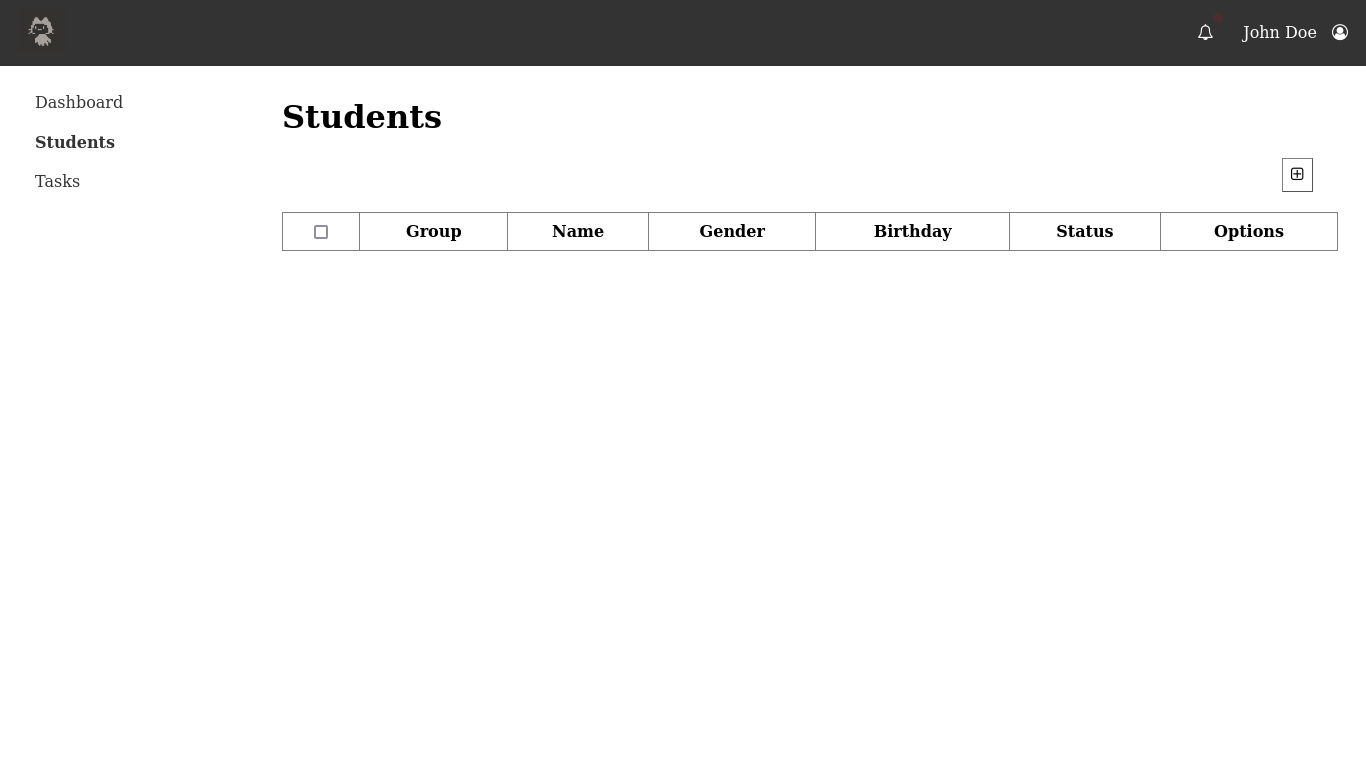
\includegraphics[scale=0.35]{1}
	\caption{Загальний вигляд сторінки}
\end{figure}

\begin{figure}[H]
	\centering
	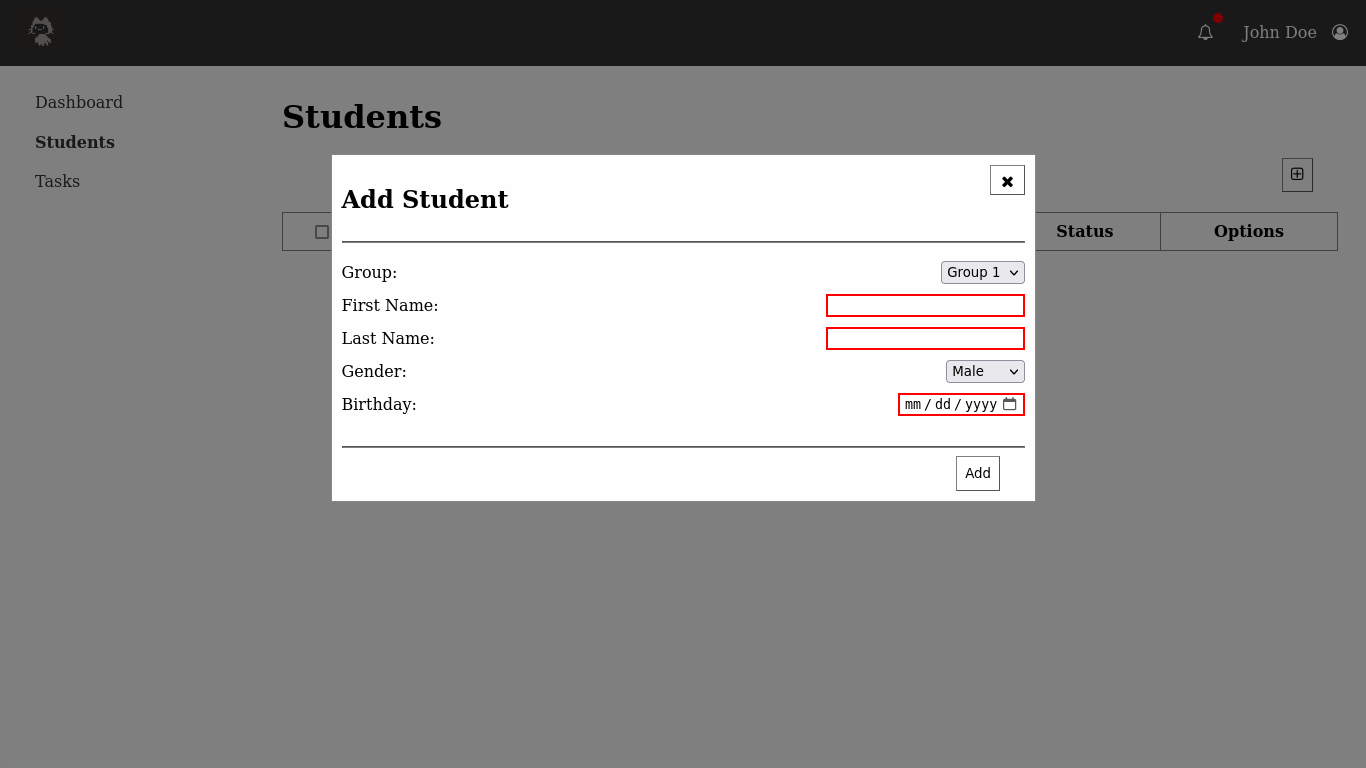
\includegraphics[scale=0.35]{3}
	\caption{Модальне вікно для додавання студента та його валідація}
\end{figure}

\begin{figure}[H]
	\centering
	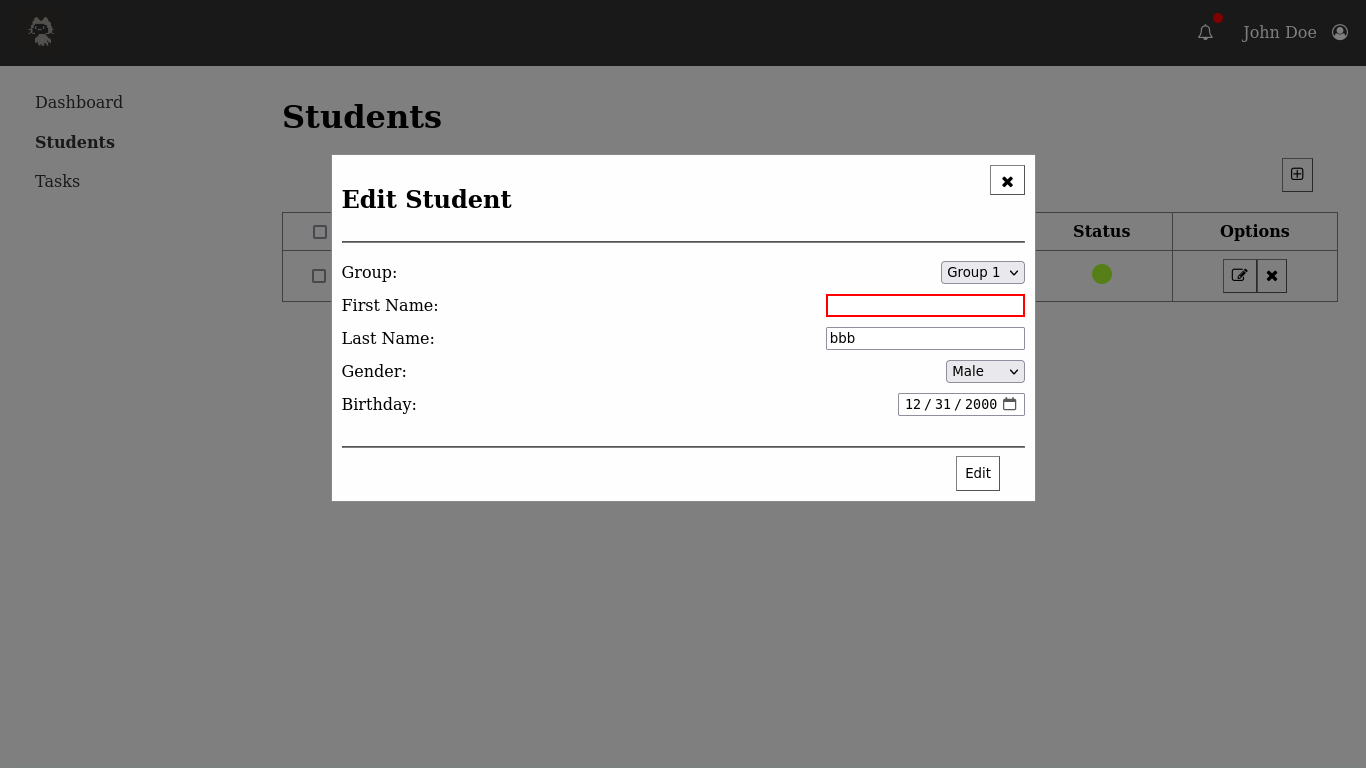
\includegraphics[scale=0.35]{6}
	\caption{Модальне вікно для видалення студента та його валідація}
\end{figure}

\begin{figure}[H]
	\centering
	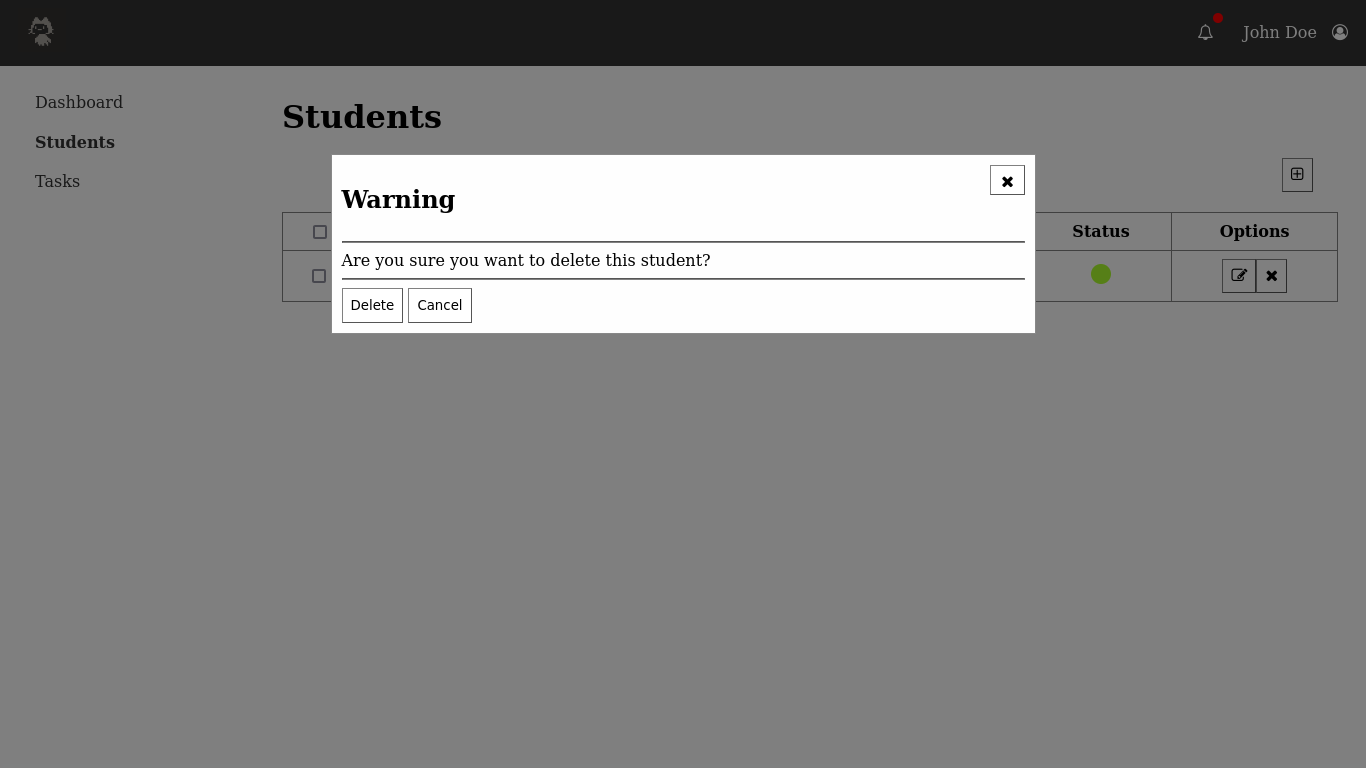
\includegraphics[scale=0.35]{7}
	\caption{Модальне вікно для видалення студента}
\end{figure}

\section*{Висновки}
Під час виконання лабораторної роботи я засвоїв елементи створення, модифікації, читання та занесення даних з
таблиць БД засобами РНР.
	    
\end{normalsize}
\end{document}
